\normaltrue \difficilefalse \tdifficilefalse
\correctionfalse

%\UPSTIidClasse{11} % 11 sup, 12 spé
%\newcommand{\UPSTIidClasse}{12}

\exer{Pompe à pistons radiaux  $\star$ \label{B2:13:11}}
\setcounter{question}{0}\UPSTIcompetence[2]{B2-13}
\index{Compétence B2-13}
\index{Pompe à pistons radiaux}
\index{Arbre à cames}
\ifcorrection
\else
\textbf{Pas de corrigé pour cet exercice.}
\fi

\ifprof
\else
Soit le mécanisme suivant. On a $\vect{AB}=e\vect{i_1}$ et $\vect{BI}=R\vect{j_0}$. De plus, 
$e=\SI{10}{mm}$ et $R=\SI{20}{mm}$. Le contact entre \textbf{1} et \textbf{2} en $B$ est maintenu en permanence par un ressort suffisamment raide (non représenté) positionné entre \textbf{0} et \textbf{2}. 
\begin{center}
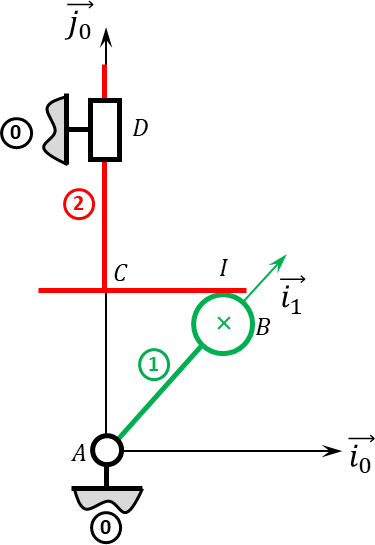
\includegraphics[width=\linewidth]{11_01}
\end{center}
\fi

Il est possible de mettre la loi entrée-sortie sous la forme *** (voir exercice \ref{C2:06:11}).

\question{Donner le torseur cinématique $\torseurcin{V}{2}{0}$ au point $B$.}
\ifprof
\else
\fi

\question{Déterminer $\vectg{B}{2}{0}$.}
\ifprof
\else
\fi

\ifprof
\else
\begin{flushright}
\footnotesize{Corrigé  voir \ref{B2:13:11}.}
\end{flushright}%
\fi